\section{AFD Palabras que contienen 'web' y/o 'ebay'}
	\subsection{Descripción del problema}
	Cosas chidas
	\begin{figure}[H]
		\begin{center}
		\includegraphics[width=14cm, height=7cm]{img/webay.png}
		\caption{Diagrama de transiciones del autómata 'webay'.}
		\label{fig:diagrama1}
		\end{center}
	\end{figure}
	\subsection{Código}
	El código fue realizado en Python 3.5.
	\\Archivo: main\_webay.py
	\begin{lstlisting}[language=Python]
	print('main_webay.py')
	\end{lstlisting}
	\\Archivo: automata\_webay.py
	\begin{lstlisting}[language=Python]
	print('automata_webay.py')
	\end{lstlisting}
	\\Archivo: diagrama\_webay.py
	\begin{lstlisting}[language=Python]
	print('diagrama_webay.py')
	\end{lstlisting}
	\subsection{Pruebas}
	Pruebas de las opciones del menú.
	\\
	{\large Modo de consola.}
	\begin{figure}[H]
		\begin{center}
			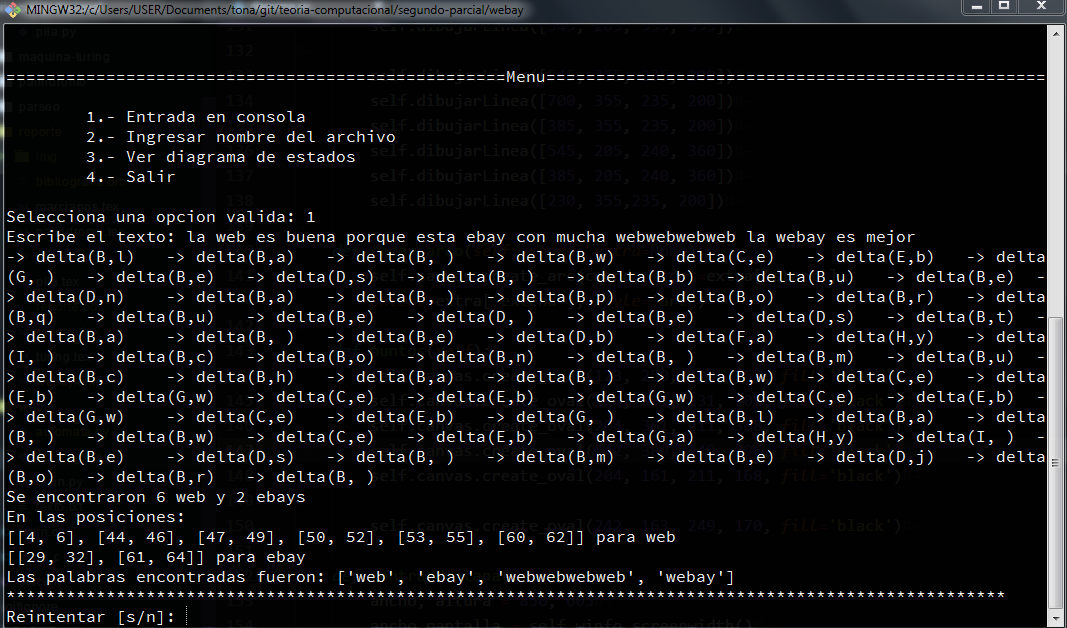
\includegraphics[width=\linewidth, height=6cm]{img/webay-manual.png}
			\caption{Historia del autómata y las palabras con 'web' y/o 'ebay'.}
			\label{fig:webay1}
		\end{center}
	\end{figure}
	{\large Modo archivo.}
	\begin{figure}[H]
		\begin{center}
			\includegraphics[width=\linewidth, height=20cm]{img/webay-automatico.png}
			\caption{Parte de la historia del autómata y las palabras con 'web' y/o 'ebay'.}
			\label{fig:webay2}
		\end{center}
	\end{figure}
	{\large Diagrama.}
	\begin{figure}[H]
		\begin{center}
			\includegraphics[width=\linewidth, height=9cm]{img/diagrama-webay.png}
			\caption{Diagrama de transiciones del autómata 'webay'.}
			\label{fig:webay3}
		\end{center}
	\end{figure}